\section{Editor}

Di seguito vengono elencati i casi d'uso per l'editor.

\subsection{Casi d'Uso}


\subsubsection{UC-E0}

    \begin{figure}[H]
      \begin{center}
        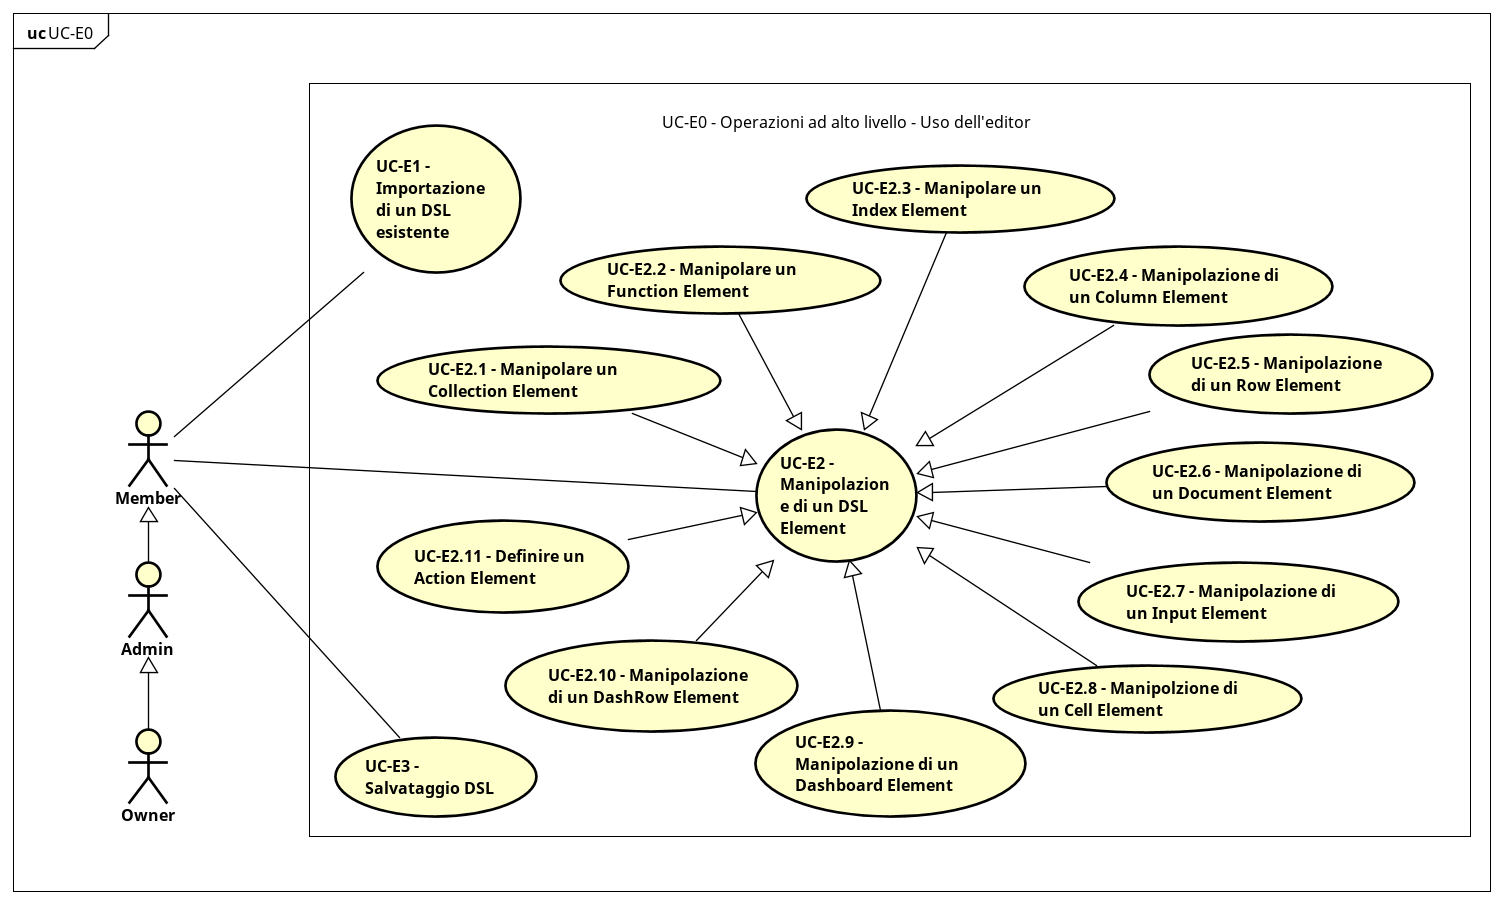
\includegraphics[width=12cm]{res/img/UCEditor/UC-E0.png}
      \caption{UC-E0 - Operazioni ad alto livello - Uso dell'editor}
      \end{center} 
    \end{figure}    
    
    %Tabella 
    \begin{center}
      \bgroup
      \def\arraystretch{1.8}     
      \begin{longtable}{  p{3.5cm} | p{8cm} } 
        
        \hline
        \multicolumn{2}{ | c | }{ \cellcolor[gray]{0.9} \textbf{UC-E0 - Operazioni ad alto livello - Uso dell'editor}} \\ 
        \hline
        
        \textbf{Attori Primari} & Utente Autenticato, Ospite, Membro, Admin, Owner \\ 
        \textbf{Scopo e Descrizione} & L'utente visualizza l'interfaccia dell'Editor tramite cui puo\` svolgere operazioni di importazione di DSL esistenti, manipolazione dei DSL Element e salvataggio del DSL corrente
        \\
        \textbf{Precondizioni}  & L'applicazione dispone l'interfaccia grafica dell'Editor \\ 
        
        \textbf{Postcondizioni} & L'utente ha utilizzato l'editor ed ha eseguito le azioni volute \\ 
        \textbf{Scenario principale} & 1. L'utilizzatore pu\`o importare un DSL esistente. (UC-E1)
2. L'utente pu\`o manipolare un DSL element. (UC-E2)
3. L'utente pu\`o salvare il DSL. (UC-E3)
      \end{longtable}
      \egroup
    \end{center}

    \subsubsection{UC-E1}    
    
    %Tabella 
    \begin{center}
      \bgroup
      \def\arraystretch{1.8}     
      \begin{longtable}{  p{3.5cm} | p{8cm} } 
        
        \hline
        \multicolumn{2}{ | c | }{ \cellcolor[gray]{0.9} \textbf{UC-E1 - Importazione di un DSL esistente}} \\ 
        \hline
        
        \textbf{Attori Primari} & Utente Autenticato, Ospite, Membro, Admin, Owner \\ 
        \textbf{Scopo e Descrizione} & L'utente pu\`o importare un DSL esistente tra quelli personali o quelli della Company. \\ 
        
        \textbf{Precondizioni}  & L'applicazione fornisce la lista di DSL tra cui scegliere quello da importare. \\ 
        
        \textbf{Postcondizioni} & L'applicazione ha caricato con successo il DSL richiesto dall'utente.
      \end{longtable}
      \egroup
    \end{center} 


\subsubsection{UC-E2}

    \begin{figure}[H]
      \begin{center}
        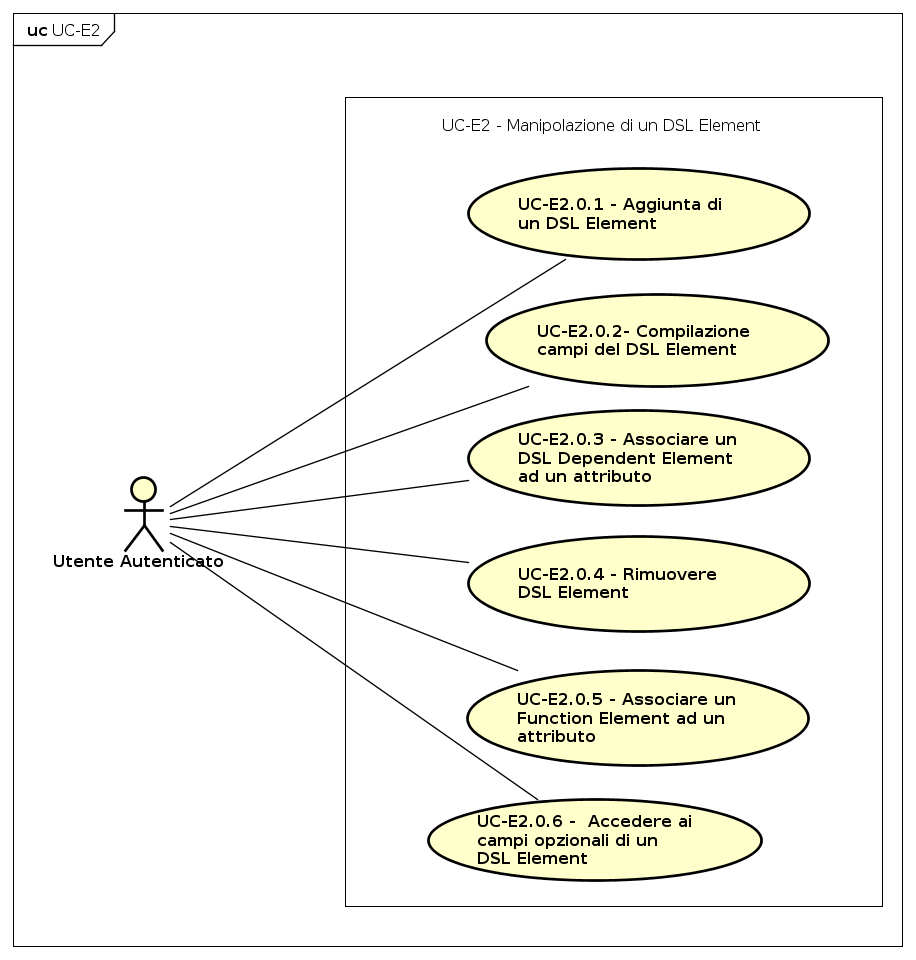
\includegraphics[width=12cm]{res/img/UCEditor/UC-E2.png}
      \caption{UC-E2 - DSL Element}
      \end{center} 
    \end{figure}    
    
    %Tabella 
    \begin{center}
      \bgroup
      \def\arraystretch{1.8}     
      \begin{longtable}{  p{3.5cm} | p{8cm} } 
        
        \hline
        \multicolumn{2}{ | c | }{ \cellcolor[gray]{0.9} \textbf{UC-E2 - Manipolazione di un DSL Element}} \\ 
        \hline
        
        \textbf{Attori Primari} & Utente Autenticato, Ospite, Membro, Admin, Owner \\ 
        \textbf{Scopo e Descrizione} & L'utente pu\`o creare, manipolare o rimuovere un DSL Element all'interno dell'editor. \\ 
        
        \textbf{Precondizioni}  & L'utente visualizza l'editor. \\ 
        
        \textbf{Postcondizioni} & L'utente ha eseguito le sue operazioni sul DSL Element con successo. \\ 
        \textbf{Scenario Principale} & 1. L'utente pu\`o aggiungere un DSL Element. (UC-E2.0.1)
2. L'attore pu\`o compilare i campi informativi del DSL Element. (UC-E2.0.2)
3. L'utente pu\`o collegare un DSL Dependent Element ad un attributo. (UC-E2.0.3)
4. L'utente ha la possibilit\`a di rimuovere un DSL Element. (UC-E2.0.4)
5. L'utente ha la possibilit\`a di associare un Function Element al DSL Element. (UC-E2.0.5)
6. L'utente ha la possibilit\`a di accedere ai campi opzionali di un DSL Element. (UC-E2.0.6)
      \end{longtable}
      \egroup
    \end{center} 


\subsubsection{UC-E2.0.1}   
    
    %Tabella 
    \begin{center}
      \bgroup
      \def\arraystretch{1.8}     
      \begin{longtable}{  p{3.5cm} | p{8cm} } 
        
        \hline
        \multicolumn{2}{ | c | }{ \cellcolor[gray]{0.9} \textbf{UC-E2.0.1 - Aggiunta di un DSL Element}} \\ 
        \hline
        
        \textbf{Attori Primari} & Utente Autenticato, Ospiete, Membro, Admin, Owner \\ 
        \textbf{Scopo e Descrizione} & L'utente ha la possibiltà di aggiungere un DSL Element e di deciderne il tipo. \\ 
        
        \textbf{Precondizioni}  & L'utente visualizza l'editor. \\ 
        
        \textbf{Postcondizioni} & L'utente ha aggiunto con successo un DSL Element.
      \end{longtable}
      \egroup
    \end{center} 
    
\subsubsection{UC-E2.0.2}

    %Tabella 
    \begin{center}
      \bgroup
      \def\arraystretch{1.8}     
      \begin{longtable}{  p{3.5cm} | p{8cm} } 
        
        \hline
        \multicolumn{2}{ | c | }{ \cellcolor[gray]{0.9} \textbf{UC-E2.0.2 - Compilazione campi del DSL Element}} \\ 
        \hline
        
        \textbf{Attori Primari} & Utente Autenticato, Ospite, Membro, Admin, Owner \\ 
        \textbf{Scopo e Descrizione} & L'utente ha la possibilit\`a di compilare i campi informativi del DSL Element. \\ 
        
        \textbf{Precondizioni}  & L'utente visualizza un DSL Element. \\ 
        
        \textbf{Postcondizioni} & Le informazioni desiderate dall'utente sono stati aggiunte nel DSL Element.
      \end{longtable}
      \egroup
    \end{center}
    
\subsubsection{UC-E2.0.3}

    %Tabella 
    \begin{center}
      \bgroup
      \def\arraystretch{1.8}     
      \begin{longtable}{  p{3.5cm} | p{8cm} } 
        
        \hline
        \multicolumn{2}{ | c | }{ \cellcolor[gray]{0.9} \textbf{UC-E2.0.3 - Associare un DSL Dependent Element ad un attributo}} \\ 
        \hline
        
        \textbf{Attori Primari} & Utente Autenticato, Ospiete, Membro, Admin, Owner \\ 
        \textbf{Scopo e Descrizione} & L'utente ha la possibilit\`a di associare un DSL Dependent Element ad un attributo. \\ 
        
        \textbf{Precondizioni}  & L'utente ha a seleziona un attributo e un DSL Dependent Element da associare. \\ 
        
        \textbf{Postcondizioni} & L'utente ha collegato con successo l'attributo e il DSL Dependent Element.
      \end{longtable}
      \egroup
    \end{center}
\subsubsection{UC-E2.0.4}

    %Tabella 
    \begin{center}
      \bgroup
      \def\arraystretch{1.8}     
      \begin{longtable}{  p{3.5cm} | p{8cm} } 
        
        \hline
        \multicolumn{2}{ | c | }{ \cellcolor[gray]{0.9} \textbf{UC-E2.0.4 - Rimuovere un DSL Element}} \\ 
        \hline
        
        \textbf{Attori Primari} & Utente Autenticato, Ospite, Membro, Admin, Owner \\ 
        \textbf{Scopo e Descrizione} & \`E possibile rimuovere un DSL Element. \\ 
        
        \textbf{Precondizioni}  & L'utente sta visualizzando l'editor e il DSL Element che vuole eliminare \`e presente nell'interfaccia dell'editor. \\ 
        
        \textbf{Postcondizioni} & L'utente ha eliminato con successo il DSL Element selezionato.
      \end{longtable}
      \egroup
    \end{center}
\subsubsection{UC-E2.0.5}

    %Tabella 
    \begin{center}
      \bgroup
      \def\arraystretch{1.8}     
      \begin{longtable}{  p{3.5cm} | p{8cm} } 
        
        \hline
        \multicolumn{2}{ | c | }{ \cellcolor[gray]{0.9} \textbf{UC-E2.0.5 - Associare un Function Element ad un attributo}} \\ 
        \hline
        
        \textbf{Attori Primari} & Utente Autenticato, Ospite, Membro, Admin, Owner \\ 
        \textbf{Scopo e Descrizione} & L'utente ha la possibilit\`a di associare un Function Element ad un attributo selezionabile di un DSL Element. \\ 
        
        \textbf{Precondizioni}  & L'utente visualizza il Function Element e il DSL Element a cui associarlo. \\ 
        
        \textbf{Postcondizioni} & L'utente ha associato con successo la Function Element ad un attributo del DSL Element.
      \end{longtable}
      \egroup
    \end{center}
    
    
\subsubsection{UC-E2.0.6}

    %Tabella 
    \begin{center}
      \bgroup
      \def\arraystretch{1.8}     
      \begin{longtable}{  p{3.5cm} | p{8cm} } 
        
        \hline
        \multicolumn{2}{ | c | }{ \cellcolor[gray]{0.9} \textbf{UC-E2.0.6 - Accedere ai campi opzionali di un DSL Element}} \\ 
        \hline
        
        \textbf{Attori Primari} & Utente Autenticato, Ospite, Membro, Admin, Owner \\ 
        \textbf{Scopo e Descrizione} & L'utente decide di poter aver accesso ai campi opzionali di un DSL Element e a renderli modificabili. \\ 
        
        \textbf{Precondizioni}  & L'utente sta visualizzando uno specifico DSL Element con campi opzionali. \\ 
        
        \textbf{Postcondizioni} & L'utente ha reso modificabili i campi opzionali del DSL Element. Tali campi possono essere modificati come descritto su caso d'uso UC-E2.0.2.
      \end{longtable}
      \egroup
    \end{center}
    
    
    
\subsubsection{UC-E2.1}
 

    \begin{figure}[H]
      \begin{center}
        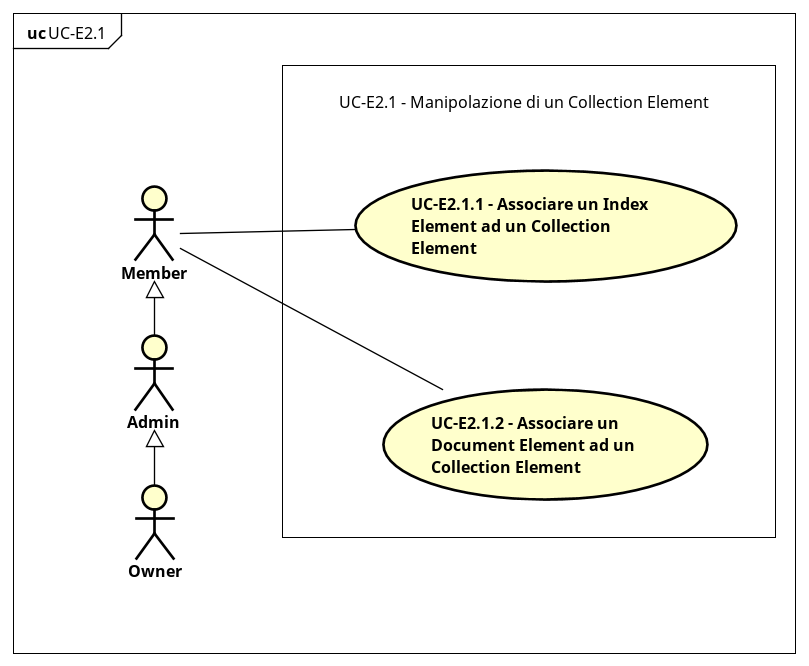
\includegraphics[width=12cm]{res/img/UCEditor/UC-E2.1.png}
      \caption{UC-E2.1 - Collection Element}
      \end{center} 
    \end{figure}

    %Tabella 
    \begin{center}
      \bgroup
      \def\arraystretch{1.8}     
      \begin{longtable}{  p{3.5cm} | p{8cm} } 
        
        \hline
        \multicolumn{2}{ | c | }{ \cellcolor[gray]{0.9} \textbf{UC-E2.1 - Manipolazione di un Collection Element}} \\ 
        \hline
        
        \textbf{Attori Primari} & Utente Autenticato, Ospite, Membro, Admin, Owner \\ 
        \textbf{Scopo e Descrizione} & L'utente pu\`o creare, manipolare o rimuovere un Collection Element all'interno dell'editor. \\ 
        
        \textbf{Precondizioni}  & L'utente sta visualizzando l'editor. \\ 
        
        \textbf{Postcondizioni} & L'utente ha manipolato il Collection Element. \\ 
        \textbf{Scenario principale} & 1. L'utente pu\`o associare un Index Element (UC-E2.1.1)
2. L'utente pu\`o associare un Document Element (UC-E2.1.2) \\
\end{longtable}
      \egroup
    \end{center}
    
    
\subsubsection{UC-E2.1.1}

    %Tabella 
    \begin{center}
      \bgroup
      \def\arraystretch{1.8}     
      \begin{longtable}{  p{3.5cm} | p{8cm} } 
        
        \hline
        \multicolumn{2}{ | c | }{ \cellcolor[gray]{0.9} \textbf{UC-E2.1.1 - Associare un Index Element ad un Collection Element}} \\ 
        \hline
        
        \textbf{Attori Primari} & Utente Autenticato, Ospite, Membro, Admin, Owner \\ 
        \textbf{Scopo e Descrizione} & L'utente ha la possibilit\`a di associare un Index Element all'attributo `index` del Collection Element \\ 
        
        \textbf{Precondizioni}  & Il Collection Element a cui associare l'Index Element \`e visualizzato nell'editor \\ 
        
        \textbf{Postcondizioni} & L'Index Element \`e stato associato ad un Collection Element
      \end{longtable}
      \egroup
    \end{center}
    
    
    
\subsubsection{UC-E2.1.2}

    %Tabella 
    \begin{center}
      \bgroup
      \def\arraystretch{1.8}     
      \begin{longtable}{  p{3.5cm} | p{8cm} } 
        
        \hline
        \multicolumn{2}{ | c | }{ \cellcolor[gray]{0.9} \textbf{UC-E2.1.2 - Associare un Document Element ad un Collection Element}} \\ 
        \hline
        
        \textbf{Attori Primari} & Utente Autenticato, Ospite, Membro, Admin, Owner \\ 
        \textbf{Scopo e Descrizione} & L'utente ha la possibilit\`a di associare un Document Element all'attributo `show` del Collection Element. \\ 
        
        \textbf{Precondizioni}  & Il Collection Element a cui associare il Document Element \`e visualizzato nell'editor.  \\ 
        
        \textbf{Postcondizioni} & Il Document Element \`e stato associato all'attributo `show` del Collection Element desiderato.
      \end{longtable}
      \egroup
    \end{center}
    
    
\subsubsection{UC-E2.2}
    \begin{figure}[H]
      \begin{center}
        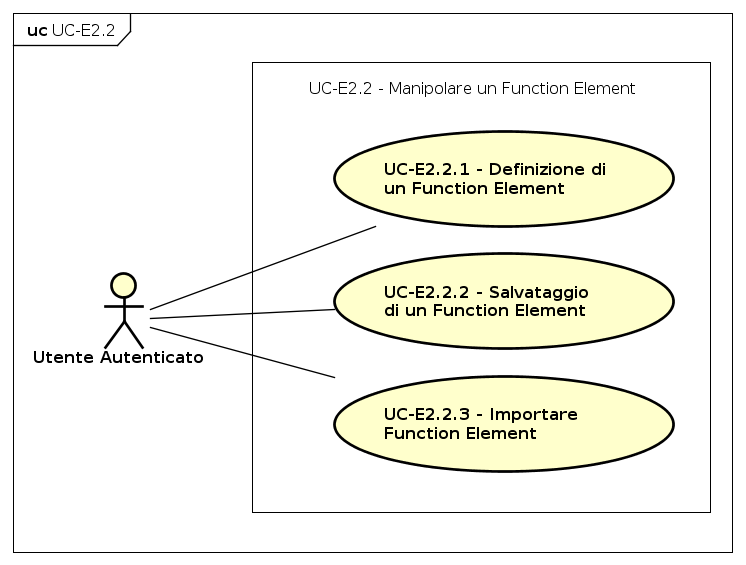
\includegraphics[width=12cm]{res/img/UCEditor/UC-E2.2.png}
      \caption{UC-E2.2 - Manipolare un Function Element}
      \end{center} 
    \end{figure}

    %Tabella 
    \begin{center}
      \bgroup
      \def\arraystretch{1.8}     
      \begin{longtable}{  p{3.5cm} | p{8cm} } 
        
        \hline
        \multicolumn{2}{ | c | }{ \cellcolor[gray]{0.9} \textbf{UC-E2.2 - Manipolare un Function Element}} \\ 
        \hline
        
        \textbf{Attori Primari} & Utente Autenticato, Ospite, Membro, Admin, Owner \\ 
        \textbf{Scopo e Descrizione} & Viene data la possibilit\`a all'utente di creare 
            un Function Element collegabile ad un attributo del DSL Element. \\ 
        
        \textbf{Precondizioni}  & L'editor \`e pronto per l'utilizzo. \\ 
        
        \textbf{Postcondizioni} & L'utente ha creato, modificato o rimosso uno specifico Function Element. \\ 
        \textbf{Scenario principale} & 1. L'utente ha la possibilit\`a di definire un \textit{function element} (UC-E2.2.1)
2. L'utente ha la possibilit\`a di salvare Function Element (UC-E2.2.2)
3. L'utente ha la possibilit\`a di importare Function Element (UC-E2.2.3)  \\
      \end{longtable}
      \egroup
    \end{center}
\subsubsection{UC-E2.2.1}

    %Tabella 
    \begin{center}
      \bgroup
      \def\arraystretch{1.8}     
      \begin{longtable}{  p{3.5cm} | p{8cm} } 
        
        \hline
        \multicolumn{2}{ | c | }{ \cellcolor[gray]{0.9} \textbf{UC-E2.2.1 - Definizione di un Function Element}} \\ 
        \hline
        
        \textbf{Attori Primari} & Utente Autenticato, Ospite, Membro, Admin, Owner \\ 
        \textbf{Scopo e Descrizione} & L'utente ha la possibilit\`a di definire all'interno di un Function Element una funzione nella sintassi del \textit{DSL}. \\ 
        
        \textbf{Precondizioni}  & L'utente sta visualizzando il form di compilazione di un Function Element. \\ 
        
        \textbf{Postcondizioni} & L'utente ha definito con successo una funzione per il Function Element.
      \end{longtable}
      \egroup
    \end{center}
\subsubsection{UC-E2.2.2}

    %Tabella 
    \begin{center}
      \bgroup
      \def\arraystretch{1.8}     
      \begin{longtable}{  p{3.5cm} | p{8cm} } 
        
        \hline
        \multicolumn{2}{ | c | }{ \cellcolor[gray]{0.9} \textbf{UC-E2.2.2 - Salvataggio di un Function Element}} \\ 
        \hline
        
        \textbf{Attori Primari} & Utente Autenticato, Ospite, Membro, Admin, Owner \\ 
        \textbf{Scopo e Descrizione} & L'utente ha la possibilit\`a di salvare il Function Element creato. \\ 
        
        \textbf{Precondizioni}  & L'utente ha inserito un Function Element valido \\ 
        
        \textbf{Postcondizioni} & Il Function Element \`e stata salvato con successo nel sistema.
      \end{longtable}
      \egroup
    \end{center}
    
    
\subsubsection{UC-E2.2.3}

    %Tabella 
    \begin{center}
      \bgroup
      \def\arraystretch{1.8}     
      \begin{longtable}{  p{3.5cm} | p{8cm} } 
        
        \hline
        \multicolumn{2}{ | c | }{ \cellcolor[gray]{0.9} \textbf{UC-E2.2.3 - Importare un Function Element}} \\ 
        \hline
        
        \textbf{Attori Primari} & Utente Autenticato, Ospite, Membro, Admin, Owner \\ 
        \textbf{Scopo e Descrizione} & Il sistema permette di importare un \textit{Function Element} precedentemente definito.\\ 
        
        \textbf{Precondizioni}  & Il sistema fornisce i \textit{Function Element} salvati nel sistema. \\ 
        
        \textbf{Postcondizioni} & L'utente ha caricato il Function Element con successo. \\ 
      \end{longtable}
      \egroup
    \end{center}
    
    
\subsubsection{UC-E2.3}
    \begin{figure}[H]
      \begin{center}
        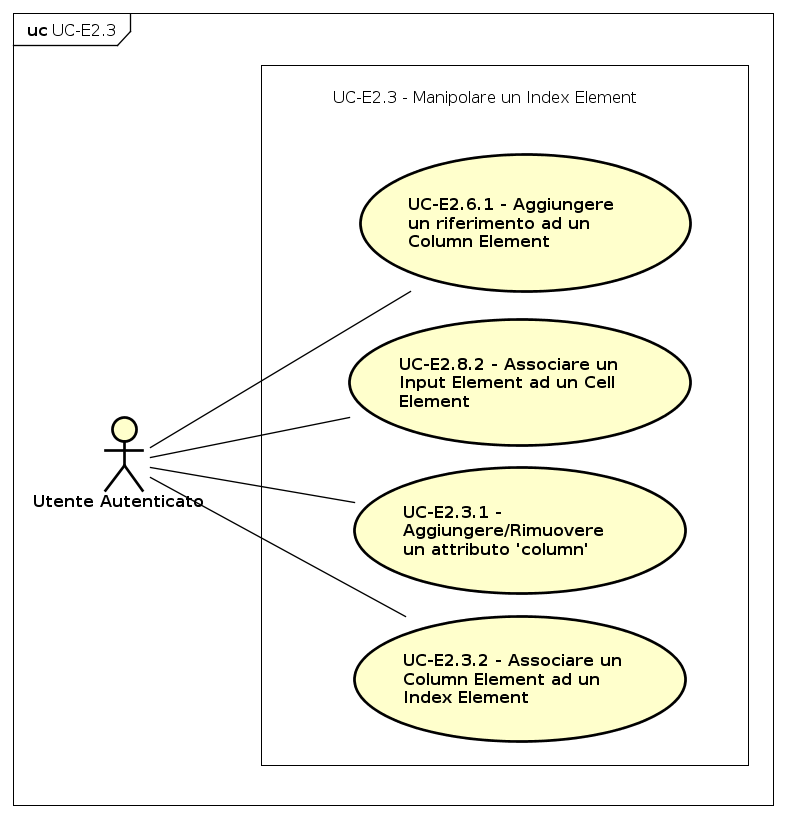
\includegraphics[width=12cm]{res/img/UCEditor/UC-E2.3.png}
      \caption{UC-E2.3 - Index Element}
      \end{center} 
    \end{figure}

    %Tabella 
    \begin{center}
      \bgroup
      \def\arraystretch{1.8}     
      \begin{longtable}{  p{3.5cm} | p{8cm} } 
        
        \hline
        \multicolumn{2}{ | c | }{ \cellcolor[gray]{0.9} \textbf{UC-E2.3 - Manipolare un Index Element}} \\ 
        \hline
        
        \textbf{Attori Primari} & Utente Autenticato, Ospite, Membro, Admin, Owner \\ 
        \textbf{Scopo e Descrizione} & L'utente ha la possibilit\`a di aggiungere, modificare o eliminare un Index Element \\ 
        
        \textbf{Precondizioni}  & L'utente \`e all'interno dell'editor. \\ 
        
        \textbf{Postcondizioni} & \`E stato manipolato l'Index Element secondo le opzioni indicatre dall'utente. \\ 
        \textbf{Scenario Principale} & 1. L'utente pu\`o aggiungere un riferimento ad un Column Element. (UC-E2.6.1)
2. L'utente pu\`o associare un Input Element. (UC-E2.8.2)
3. L'utente pu\`o aggiungere/rimuovere un attributo ``column''. (UC-E2.3.1)
4. L'utente ha la possibilit\'a di associare un Column Element. (UC-E2.3.2)
      \end{longtable}
      \egroup
    \end{center}
\subsubsection{UC-E2.3.1}

    %Tabella 
    \begin{center}
      \bgroup
      \def\arraystretch{1.8}     
      \begin{longtable}{  p{3.5cm} | p{8cm} } 
        
        \hline
        \multicolumn{2}{ | c | }{ \cellcolor[gray]{0.9} \textbf{UC-E2.3.1 - Aggiungere/Rimuovere un attributo ``column''}} \\ 
        \hline
        
        \textbf{Attori Primari} & Utente Autenticato, Ospite, Membro, Admin, Owner \\ 
        \textbf{Scopo e Descrizione} & L'utente ha la possibilit\`a di rimuovere o aggiungere dall'Index Element un attributo ``column''. \\ 
        
        \textbf{Precondizioni}  &  L'utente \`e all'interno dell'editor e sta visualizzando un Index Element da modificare. \\ 
        
        \textbf{Postcondizioni} & Il sistema aggiunge un attributo ``column'' all'Index Element modificato.
      \end{longtable}
      \egroup
    \end{center}
\subsubsection{UC-E2.3.2}

    %Tabella 
    \begin{center}
      \bgroup
      \def\arraystretch{1.8}     
      \begin{longtable}{  p{3.5cm} | p{8cm} } 
        
        \hline
        \multicolumn{2}{ | c | }{ \cellcolor[gray]{0.9} \textbf{UC-E2.3.2 - Associare un \textit{Column Element} ad un Index Element}} \\ 
        \hline
        
        \textbf{Attori Primari} & Utente Autenticato, Ospite, Membro, Admin, Owner \\ 
        \textbf{Scopo e Descrizione} & L'utente ha la possibilit\`a di associare un Column Element ad un attributo ``column'' di un Index Element. \\ 
        
        \textbf{Precondizioni}  & L'utente visualizza un Index Element su cui associare il Column Element. \\ 
        
        \textbf{Postcondizioni} & Il sistema associa correttamente il Column Element all Index Element indicato dall'utente.
      \end{longtable}
      \egroup
    \end{center}
    
    
\subsubsection{UC-E2.4}

    %Tabella 
    \begin{center}
      \bgroup
      \def\arraystretch{1.8}     
      \begin{longtable}{  p{3.5cm} | p{8cm} } 
        
        \hline
        \multicolumn{2}{ | c | }{ \cellcolor[gray]{0.9} \textbf{UC-E2.4 - Manipolazione di un Column Element}} \\ 
        \hline
        
        \textbf{Attori Primari} & Utente Autenticato, Ospite, membro, Admin, Owner \\ 
        \textbf{Scopo e Descrizione} & L'utente ha la possibilit\`a di aggiungere, rimuovere o modificare un Column Element \\ 
        
        \textbf{Precondizioni}  & L'editor \`e visualizzato dall'utente. \\ 
        
        \textbf{Postcondizioni} & Il sistema compie le operazioni sul Column Element indicato dall'utente.
      \end{longtable}
      \egroup
    \end{center}
    
\subsubsection{UC-E2.5}

    %Tabella 
    \begin{center}
      \bgroup
      \def\arraystretch{1.8}     
      \begin{longtable}{  p{3.5cm} | p{8cm} } 
        
        \hline
        \multicolumn{2}{ | c | }{ \cellcolor[gray]{0.9} \textbf{UC-E2.5 - Manipolazione di Row Element}} \\ 
        \hline
        
        \textbf{Attori Primari} & Utente Autenticato, Ospite, Membro, Admin, Owner \\ 
        \textbf{Scopo e Descrizione} & L'utente ha la possibilit\`a di aggiungere, rimuovere o modificare un Row Element \\ 
        
        \textbf{Precondizioni}  & L'editor \`e visualizzato dall'utente. \\ 
        
        \textbf{Postcondizioni} & Il sistema compie le operazioni sul Column Element indicato dall'utente.
      \end{longtable}
      \egroup
    \end{center}
\subsubsection{UC-E2.6}
 

    \begin{figure}[H]
      \begin{center}
        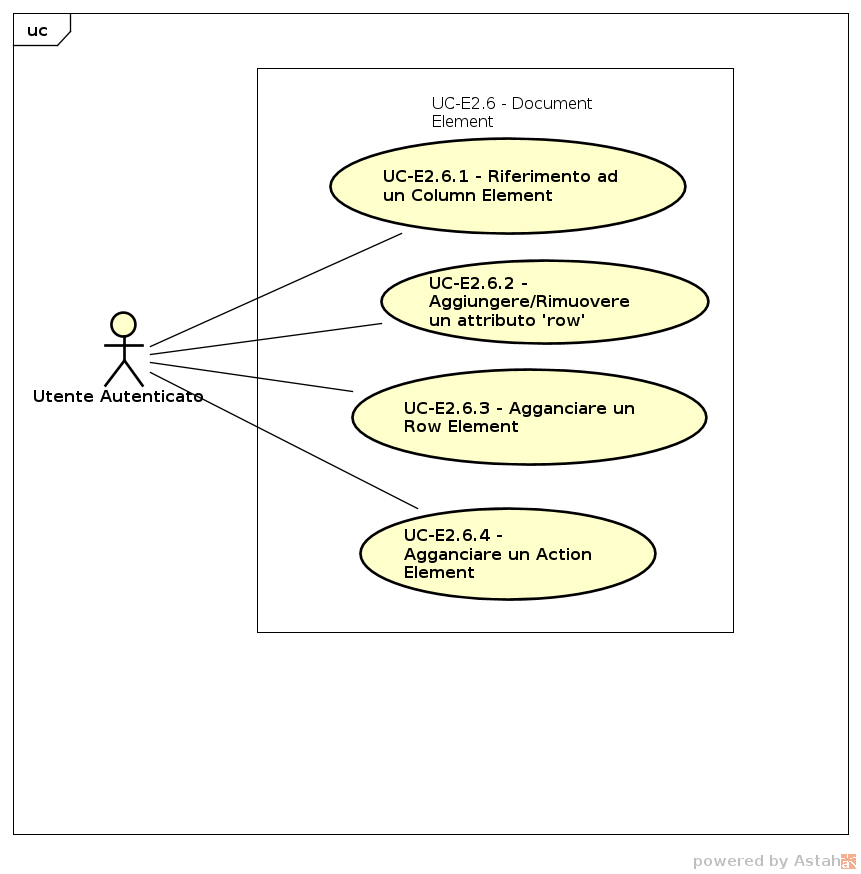
\includegraphics[width=12cm]{res/img/UCEditor/UC-E2.6-DocumentElement}
      \caption{UC-E2.6 - Document Element}
      \end{center} 
    \end{figure}

    %Tabella 
    \begin{center}
      \bgroup
      \def\arraystretch{1.8}     
      \begin{longtable}{  p{3.5cm} | p{8cm} } 
        
        \hline
        \multicolumn{2}{ | c | }{ \cellcolor[gray]{0.9} \textbf{UC-E2.6 - Manipulare un Document Element}} \\ 
        \hline
        
        \textbf{Attori Primari} & Utente Autenticato, Ospite, Membro, Admin, Owner \\ 
        \textbf{Scopo e Descrizione} & L'editor offre la possibilit\`a di manipulare un Document Element agganciandogli altri elementi \\ 
        
        \textbf{Precondizioni}  & L'utente visualizza l'editor \\ 
        
        \textbf{Postcondizioni} & Viene generato l'elemento Document nel DSL \\ 
        \textbf{Scenario Principale} & 1. L'utente ha la possibilit\`a di aggiungere un riferimento ad un Column Element. (UC-E2.6.1)
2. L\`utente pu\`o aggiungere/aimuovere un attributo row. (UC-E2.6.2)
3. L\`utente pu\`o associare un Row Element. (UC-E2.6.3)
4. L\`utente pu\`o associare agganciare un Action Element. (UC-E2.6.4) 
      \end{longtable}
      \egroup
    \end{center}
\subsubsection{UC-E2.6.1}

    %Tabella 
    \begin{center}
      \bgroup
      \def\arraystretch{1.8}     
      \begin{longtable}{  p{3.5cm} | p{8cm} } 
        
        \hline
        \multicolumn{2}{ | c | }{ \cellcolor[gray]{0.9} \textbf{UC-E2.6.1 - Aggiungere un riferimento ad un Column Element}} \\ 
        \hline
        
        \textbf{Attori Primari} & Utente Autenticato, Ospite, Membro, Admin, Owner \\ 
        \textbf{Scopo e Descrizione} & Si da la possibilit\`a di aggiungere una \glossaryItem{associazione per riferimento} tra il Column Element e l'attributo populate del Document Element. \\ 
        
        \textbf{Precondizioni}  & Il Document Element esiste nella sessione corrente dell'editor \\ 
        
        \textbf{Postcondizioni} & Il sistema aggiunge un riferimento tra il Column Element e il Document Element.
      \end{longtable}
      \egroup
    \end{center}
    
    
\subsubsection{UC-E2.6.2}

    %Tabella 
    \begin{center}
      \bgroup
      \def\arraystretch{1.8}     
      \begin{longtable}{  p{3.5cm} | p{8cm} } 
        
        \hline
        \multicolumn{2}{ | c | }{ \cellcolor[gray]{0.9} \textbf{UC-E2.6.2 - Aggiungere/Rimuovere un attributo Row}} \\ 
        \hline
        
        \textbf{Attori Primari} & Utente Autenticato, Ospite, Membro, Admin, Owner \\ 
        \textbf{Scopo e Descrizione} & Il sistema dispone la possibilit\`a di aggiungere o rimuovere un attributo Row da un Document Element. \\ 
        
        \textbf{Precondizioni}  & Il Document Element su cui operare l'aggiunta/rimozione di un attributo Row esiste nella sessione corrente dell'editor. \\ 
        
        \textbf{Postcondizioni} & \`E stata manipolata (aggiunta o rimossa) un attributo Row all'interno del DSL Document.
      \end{longtable}
      \egroup
    \end{center}
\subsubsection{UC-E2.6.3}

    %Tabella 
    \begin{center}
      \bgroup
      \def\arraystretch{1.8}     
      \begin{longtable}{  p{3.5cm} | p{8cm} } 
        
        \hline
        \multicolumn{2}{ | c | }{ \cellcolor[gray]{0.9} \textbf{UC-E2.6.3 - Associare un Row Element ad un attributo Row}} \\ 
        \hline
        
        \textbf{Attori Primari} & Utente Autenticato, Ospite, Membro, Admin, Owner \\ 
        \textbf{Scopo e Descrizione} & Il sistema dispone la funzionalit\`a di aggiungere un'associazione tra un Row Element e un attributo Row di uno specifico Document Element.  \\ 
        
        \textbf{Precondizioni}  & Il Document Element e il Row Element decisi dall'utente esistono nella sessione corrente dell'editor. \\ 
        
        \textbf{Postcondizioni} & Il sistema ha creato l'associazione tra il Row Element e l'attributo Row del Document Element scelto.
      \end{longtable}
      \egroup
    \end{center}
\subsubsection{UC-E2.6.4}

    %Tabella 
    \begin{center}
      \bgroup
      \def\arraystretch{1.8}     
      \begin{longtable}{  p{3.5cm} | p{8cm} } 
        
        \hline
        \multicolumn{2}{ | c | }{ \cellcolor[gray]{0.9} \textbf{UC-E2.6.4 - Associare un Action Element}} \\ 
        \hline
        
        \textbf{Attori Primari} & Utente Autenticato, Ospite, Membro, Admin, Owner \\ 
        \textbf{Scopo e Descrizione} & Il sistema dispone la funzionalit\`a di associare un Action Element ad un attributo Row di un Document Element. \\ 
        
        \textbf{Precondizioni}  & Il Document Element con il relativo attributo Row esistono nella sessione corrente. \\ 
        
        \textbf{Postcondizioni} & Viene creata un'associazione tra Action Element e l'attributo Row del Document Element indicato dall'utente. 
      \end{longtable}
      \egroup
    \end{center}
\subsubsection{UC-E2.7}
 

    \begin{figure}[H]
      \begin{center}
        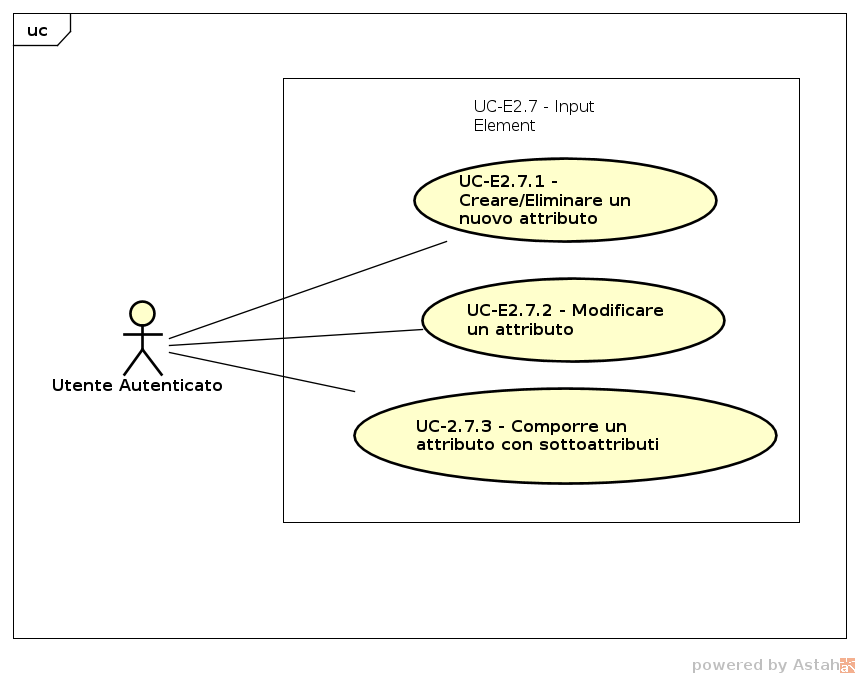
\includegraphics[width=12cm]{res/img/UCEditor/UC-E2.7-InputElement}
      \caption{UC-E2.7 - Input Element}
      \end{center} 
    \end{figure}

    %Tabella 
    \begin{center}
      \bgroup
      \def\arraystretch{1.8}     
      \begin{longtable}{  p{3.5cm} | p{8cm} } 
        
        \hline
        \multicolumn{2}{ | c | }{ \cellcolor[gray]{0.9} \textbf{UC-E2.7 - Manipolare un Input Element}} \\ 
        \hline
        
        \textbf{Attori Primari} & Utente Autenticato, Ospite, Membro, Admin, Owner \\ 
        \textbf{Scopo e Descrizione} & Il sistema da la possibilit\`a all'utente di modificare un Input Element agendo  sui suoi attributi.  \\ 
        
        \textbf{Precondizioni}  & L'utente si trova in una sessione dell'editor valida. \\ 
        
        \textbf{Postcondizioni} & Il sistema ha eseguito le operazioni indicate dall'utente. \\ 
        \textbf{Scenario Principale} & 1. L\`utente pu\`o creare/eliminare un nuovo attributo per l'Input Element. (UC-E2.7.1)
2. L\`utente pu\`o modificare un attributo dell'Input Element. (UC-E2.7.2)
3. L\`utente pu\`o aggiungere ad un attributo dei sottoattributi. (UC-E2.7.3)
      \end{longtable}
      \egroup
    \end{center}
\subsubsection{UC-E2.7.1}

    %Tabella 
    \begin{center}
      \bgroup
      \def\arraystretch{1.8}     
      \begin{longtable}{  p{3.5cm} | p{8cm} } 
        
        \hline
        \multicolumn{2}{ | c | }{ \cellcolor[gray]{0.9} \textbf{UC-E2.7.1 - Creare/Eliminare un nuovo attributo dell'Input Element}} \\ 
        \hline
        
        \textbf{Attori Primari} & Utente Autenticato, Ospite, Membro, Admin, Owner \\ 
        \textbf{Scopo e Descrizione} & Il sistema fornisce le operazioni di creazione ed eliminazione di un attributo di un Input Element selezionato. \\ 
        
        \textbf{Precondizioni}  & L'utente si deve riferire a un Input Element presente nella sessione corrente dell'editor. \\ 
        
        \textbf{Postcondizioni} & Il sistema agisce sull'Input Element aggiungendo o rimuovendo un attributo.
      \end{longtable}
      \egroup
    \end{center}
\subsubsection{UC-E2.7.2}

    %Tabella 
    \begin{center}
      \bgroup
      \def\arraystretch{1.8}     
      \begin{longtable}{  p{3.5cm} | p{8cm} } 
        
        \hline
        \multicolumn{2}{ | c | }{ \cellcolor[gray]{0.9} \textbf{UC-E2.7.2 - Modificare un attributo dell'Input Element}} \\ 
        \hline
        
        \textbf{Attori Primari} & Utente Autenticato, Ospite, Membro, Admin, Owner \\ 
        \textbf{Scopo e Descrizione} & L'utente ha la possibilit\`a di modificare la chiave o il valore di un attributo dell'Input Element. \\ 
        
        \textbf{Precondizioni}  & L'Input Element selezionato dall'utente possiede l'attributo da modificare. \\ 
        
        \textbf{Postcondizioni} & Il sistema ha modificato la chiave o il valore dell'attributo selezionato dall'utente.
      \end{longtable}
      \egroup
    \end{center}
\subsubsection{UC-E2.7.3}

    %Tabella 
    \begin{center}
      \bgroup
      \def\arraystretch{1.8}     
      \begin{longtable}{  p{3.5cm} | p{8cm} } 
        
        \hline
        \multicolumn{2}{ | c | }{ \cellcolor[gray]{0.9} \textbf{UC-E2.7.3 - L\`utente pu\`o aggiungere ad un attributo dei sottoattributi}} \\ 
        \hline
        
        \textbf{Attori Primari} & Utente Autenticato, Ospite, Membro, Admin, Owner \\ 
        \textbf{Scopo e Descrizione} & L'utente ha la possibilit\`a di poter definire strutture complesse associate ad un attributo. \\ 
        
        \textbf{Precondizioni}  & L'Input Element che possiede l'attributo da espandere esiste nella sessione corrente dell'editor. \\ 
        
        \textbf{Postcondizioni} & Il sistema ha memorizzato la struttura complessa associata all'attributo selezionato dall'utente.
      \end{longtable}
      \egroup
    \end{center}
\subsubsection{UC-E2.8}
 

    \begin{figure}[H]
      \begin{center}
        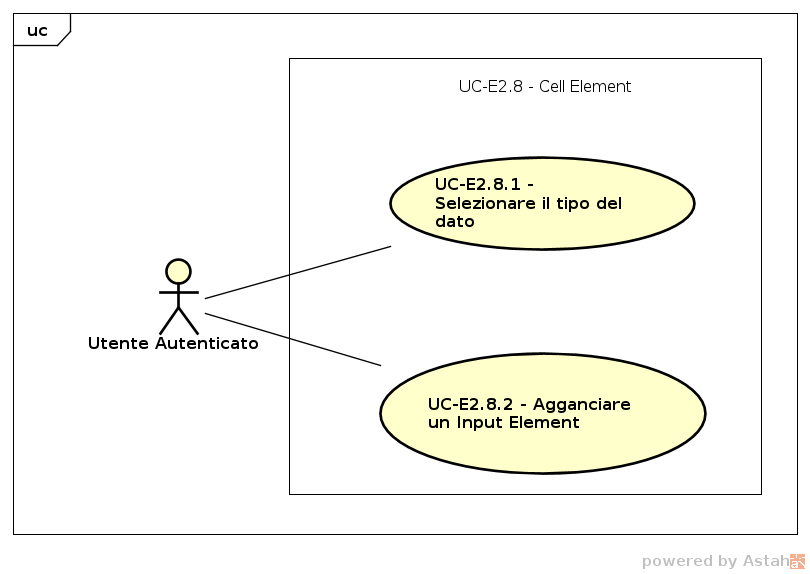
\includegraphics[width=12cm]{res/img/UCEditor/UC-E2.8-CellElement}
      \caption{UC-E2.8 - Cell Element}
      \end{center} 
    \end{figure}

    %Tabella 
    \begin{center}
      \bgroup
      \def\arraystretch{1.8}     
      \begin{longtable}{  p{3.5cm} | p{8cm} } 
        
        \hline
        \multicolumn{2}{ | c | }{ \cellcolor[gray]{0.9} \textbf{UC-E2.8 - Manipolare un Cell Element}} \\ 
        \hline
        
        \textbf{Attori Primari} & Utente Autenticato, Ospite, Membro, Admin, Owner \\ 
        \textbf{Scopo e Descrizione} & L'applicazione fornisce i metodi per definire un Cell Element valido. \\ 
        
        \textbf{Precondizioni}  & L'utente sta visualizzando l'editor. \\ 
        
        \textbf{Postcondizioni} & Il sistema espone il Cell Element valido appena definito. \\ 
        \textbf{Scenario Principale} &  1. Selezionare il tipo del dato associato al Cell Element. (UC-E2.8.1)
2. L'utente pu\`o associare un Input Element. (UC-E2.8.2)
      \end{longtable}
      \egroup
    \end{center}
    
    
    
\subsubsection{UC-E2.8.1}

    %Tabella 
    \begin{center}
      \bgroup
      \def\arraystretch{1.8}     
      \begin{longtable}{  p{3.5cm} | p{8cm} } 
        
        \hline
        \multicolumn{2}{ | c | }{ \cellcolor[gray]{0.9} \textbf{UC-E2.8.1 - Selezionare il tipo del dato associato al Cell Element}} \\ 
        \hline
        
        \textbf{Attori Primari} & Utente Autenticato, Ospite, Membro, Admin, Owner \\ 
        \textbf{Scopo e Descrizione} & L'utente pu\`o indicare il tipo di dato da visualizzare tra:
a. string;
b. number;
c. link;
d. image;
e. date. \\ 
        
        \textbf{Precondizioni}  & Il Cell Element su cui si vuole operare esiste nella sessione attiva dell'editor. \\ 
        
        \textbf{Postcondizioni} & Il sistema memorizza il tipo di dato per il Cell Element. 
      \end{longtable}
      \egroup
    \end{center}
\subsubsection{UC-E2.8.2}

    %Tabella 
    \begin{center}
      \bgroup
      \def\arraystretch{1.8}     
      \begin{longtable}{  p{3.5cm} | p{8cm} } 
        
        \hline
        \multicolumn{2}{ | c | }{ \cellcolor[gray]{0.9} \textbf{UC-E2.8.2 - Associare un Input Element ad un Cell Element}} \\ 
        \hline
        
        \textbf{Attori Primari} & Utente Autenticato, Ospite, Membro, Admin, Owner \\ 
        \textbf{Scopo e Descrizione} & Il sistema dispone l'operazione di collegamento tra un Input Element e la sua rappresentazione tramite Cell Element. \\ 
        
        \textbf{Precondizioni}  & L'Input Element e il Cell Element da collegare esistono nella sessione corrente dell'editor. \\ 
        
        \textbf{Postcondizioni} & Il sistema ha creato il collegamento tra i due elementi.
      \end{longtable}
      \egroup
    \end{center}
\subsubsection{UC-E2.9}
 

    \begin{figure}[H]
      \begin{center}
        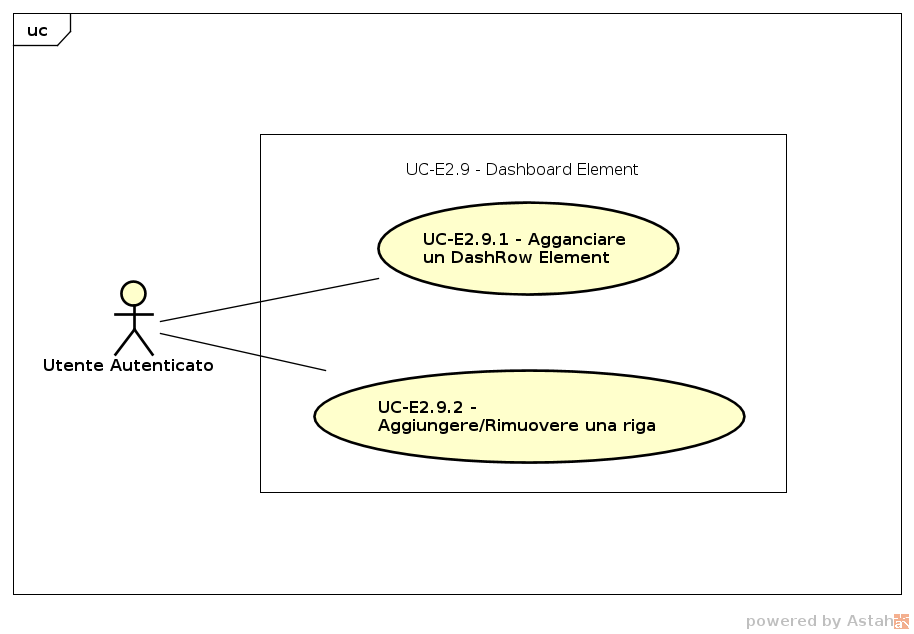
\includegraphics[width=12cm]{res/img/UCEditor/UC-E2.9-DashboardElement}
      \caption{UC-E2.9 - Dashboard Element}
      \end{center} 
    \end{figure}

    %Tabella 
    \begin{center}
      \bgroup
      \def\arraystretch{1.8}     
      \begin{longtable}{  p{3.5cm} | p{8cm} } 
        
        \hline
        \multicolumn{2}{ | c | }{ \cellcolor[gray]{0.9} \textbf{UC-E2.9 - Manipolare un Dashboard Element}} \\ 
        \hline
        
        \textbf{Attori Primari} & Utente Autenticato, Ospite, Membro, Admin, Owner \\ 
        \textbf{Scopo e Descrizione} & L'utente ha la possibilit\`a di manipolare un Dashboard Element. \\ 
        
        \textbf{Precondizioni}  & L'utente sta visualizzando l'editor. \\ 
        
        \textbf{Postcondizioni} & Il sistema ha memorizzato una definizione valida per il Dashboard Element. \\ 
        \textbf{Scenario Principale} & 1. L'utente pu\`o associare un DashRow Element ad un Dashboard Element. (UC-E2.9.1)
2. L'utente pu\`o aggiungere/rimuovere un attributo Row dal Dashboard Element. (UC-E2.9.2)
      \end{longtable}
      \egroup
    \end{center}
    
    
\subsubsection{UC-E2.9.1}

    %Tabella 
    \begin{center}
      \bgroup
      \def\arraystretch{1.8}     
      \begin{longtable}{  p{3.5cm} | p{8cm} } 
        
        \hline
        \multicolumn{2}{ | c | }{ \cellcolor[gray]{0.9} \textbf{UC-E2.9.1 - Associare un DashRow Element ad un Dashboard Element}} \\ 
        \hline
        
        \textbf{Attori Primari} & Utente Autenticato, Ospite, Membro, Admin, Owner \\ 
        \textbf{Scopo e Descrizione} & Permette di definire la struttura di una Row e di legarla a una Dashboard. \\ 
        
        \textbf{Precondizioni}  & il Dashboard Element e il DashRow Element da collegare esistono nella sessione corrente dell'editor. \\ 
        
        \textbf{Postcondizioni} & Il sistema ha memorizzato il collegamento tra l'attributo Row del Dashboard Element e il DashRow Element.
      \end{longtable}
      \egroup
    \end{center}
\subsubsection{UC-E2.9.2}

    %Tabella 
    \begin{center}
      \bgroup
      \def\arraystretch{1.8}     
      \begin{longtable}{  p{3.5cm} | p{8cm} } 
        
        \hline
        \multicolumn{2}{ | c | }{ \cellcolor[gray]{0.9} \textbf{UC-E2.9.2 - Aggiungere/Rimuovere un attributo Row dal Dashboard Element}} \\ 
        \hline
        
        \textbf{Attori Primari} & Utente Autenticato, Ospite, Membro, Admin, Owner \\ 
        \textbf{Scopo e Descrizione} & L'utente pu\`o definire una nuovo attributo Row all'interno della Dashboard \\ 
        
        \textbf{Precondizioni}  & Il Dashboard Element esiste nella sessione corrente dell'editor. \\ 
        
        \textbf{Postcondizioni} & Il sistema ha aggiunto o rimosso l'attributo Row dalla Dashboard Element. 
      \end{longtable}
      \egroup
    \end{center}
    
    
\subsubsection{UC-E2.10}
 

    \begin{figure}[H]
      \begin{center}
        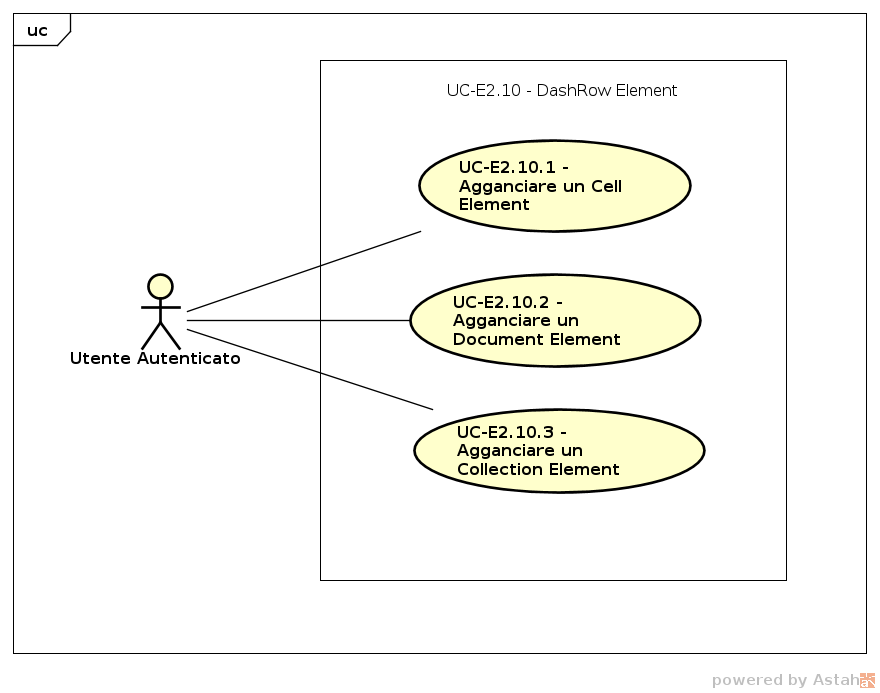
\includegraphics[width=12cm]{res/img/UCEditor/UC-E2.10-DashRowElement}
      \caption{UC-E2.10 - DashRow Element}
      \end{center} 
    \end{figure}

    %Tabella 
    \begin{center}
      \bgroup
      \def\arraystretch{1.8}     
      \begin{longtable}{  p{3.5cm} | p{8cm} } 
        
        \hline
        \multicolumn{2}{ | c | }{ \cellcolor[gray]{0.9} \textbf{UC-E2.10 - Manipolare un DashRow Element}} \\ 
        \hline
        
        \textbf{Attori Primari} & Utente Autenticato, Ospite, Membro, Admin, Owner \\ 
        \textbf{Scopo e Descrizione} & Il sistema fornisce i metodi necessari alla manipolazione di un DashRow Element. \\ 
        
        \textbf{Precondizioni}  & Il DashRow Element da manipolare esiste nella sessione corrente dell'editor. \\ 
        
        \textbf{Postcondizioni} & Il sistema ha memorizzato la configurazione del DashRow Element. \\ 
        \textbf{Scenario Principale} & 1. L'utente pu\`o associare un Cell Element al DashRow Element. (UC-E2.10.1)
2. L'utente pu\`o associare un Document Element al DashRow Element. (UC-E2.10.2)
3. L'utente pu\`o associare un Collection Element al DashRow Element. (UC-E2.10.3)
      \end{longtable}
      \egroup
    \end{center}
\subsubsection{UC-E2.10.1}

    %Tabella 
    \begin{center}
      \bgroup
      \def\arraystretch{1.8}     
      \begin{longtable}{  p{3.5cm} | p{8cm} } 
        
        \hline
        \multicolumn{2}{ | c | }{ \cellcolor[gray]{0.9} \textbf{UC-E2.10.1 - Associare un Cell Element al DashRow Element}} \\ 
        \hline
        
        \textbf{Attori Primari} & Utente Autenticato, Ospite, Membro, Admin, Owner \\ 
        \textbf{Scopo e Descrizione} & Il sistema da la possibilit\`a di associare un Cell Element ad un DashRow Element. \\ 
        
        \textbf{Precondizioni}  & Il Cell Element e il DashRow Element da associare esistono nella sessione corrente dell'editor. \\ 
        
        \textbf{Postcondizioni} & Il sistema ha memorizzato il collegamento tra i due elementi.
      \end{longtable}
      \egroup
    \end{center}
\subsubsection{UC-E2.10.2}

    %Tabella 
    \begin{center}
      \bgroup
      \def\arraystretch{1.8}     
      \begin{longtable}{  p{3.5cm} | p{8cm} } 
        
        \hline
        \multicolumn{2}{ | c | }{ \cellcolor[gray]{0.9} \textbf{UC-E2.10.2 - Associare un Document Element al DashRow Element}} \\ 
        \hline
        
        \textbf{Attori Primari} & Utente Autenticato, Ospite, Membro, Admin, Owner \\ 
        \textbf{Scopo e Descrizione} & Il sistema da la possibilit\`a di associare un Document Element ad un DashRow Element. \\ 
        
        \textbf{Precondizioni}  & Il Document Element e il DashRow Element esistono nella sessione corrente dell'editor. \\ 
        
        \textbf{Postcondizioni} & Il sistema ha memorizzato il collegamento tra i due elementi.
      \end{longtable}
      \egroup
    \end{center}
\subsubsection{UC-E2.10.3}

    %Tabella 
    \begin{center}
      \bgroup
      \def\arraystretch{1.8}     
      \begin{longtable}{  p{3.5cm} | p{8cm} } 
        
        \hline
        \multicolumn{2}{ | c | }{ \cellcolor[gray]{0.9} \textbf{UC-E2.10.3 - Associare un Collection Element ad un DashRow Element}} \\ 
        \hline
        
        \textbf{Attori Primari} & Utente Autenticato, Ospite, Membro, Admin, Owner \\ 
        \textbf{Scopo e Descrizione} & Il sistema da la possibilit\`a di associare un Collection Element ad un DashRow Element. \\ 
        
        \textbf{Precondizioni}  & Il Collection Element e il DashRow Element esistono nella sessione corrente dell'editor. \\ 
        
        \textbf{Postcondizioni} & Il sistema ha memorizzato il collegamento tra i due elementi.
      \end{longtable}
      \egroup
    \end{center}
\subsubsection{UC-E2.11}
 

    \begin{figure}[H]
      \begin{center}
        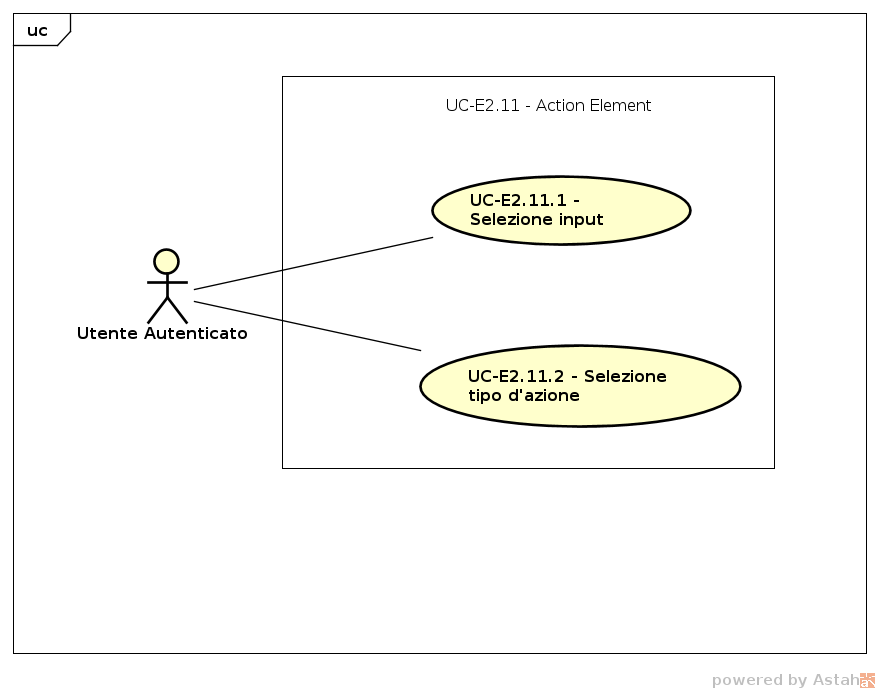
\includegraphics[width=12cm]{res/img/UCEditor/UC-E2.11-ActionElement}
      \caption{UC-E2.11 - Action Element}
      \end{center} 
    \end{figure}

    %Tabella 
    \begin{center}
      \bgroup
      \def\arraystretch{1.8}     
      \begin{longtable}{  p{3.5cm} | p{8cm} } 
        
        \hline
        \multicolumn{2}{ | c | }{ \cellcolor[gray]{0.9} \textbf{UC-E2.11 - Definire un Action Element}} \\ 
        \hline
        
        \textbf{Attori Primari} & Utente Autenticato, Ospite, Membro, Admin, Onwer \\ 
        \textbf{Scopo e Descrizione} & Il sistema fornisce le modalit\`a di definizione di un Action Element. \\ 
        
        \textbf{Precondizioni}  & L'utente sta visualizzando l'editor. \\ 
        
        \textbf{Postcondizioni} &  Il sistema ha registrato la definizione dell'Action Element. \\ 
        \textbf{Scenario Principale} & 1. L'utente seleziona un input per l'Action Element. (UC-E2.11.1)
2. L'utente seleziona il tipo d'azione per l'Action Element. (UC-E2.11.2) 
      \end{longtable}
      \egroup
    \end{center}
\subsubsection{UC-E2.11.1}

    %Tabella 
    \begin{center}
      \bgroup
      \def\arraystretch{1.8}     
      \begin{longtable}{  p{3.5cm} | p{8cm} } 
        
        \hline
        \multicolumn{2}{ | c | }{ \cellcolor[gray]{0.9} \textbf{UC-E2.11.1 - Selezione input per Action Element}} \\ 
        \hline
        
        \textbf{Attori Primari} & Utente Autenticato, Ospite, Membro, Admin, Owner \\ 
        \textbf{Scopo e Descrizione} & L'utente ha la possibilit\`a di selezionare l'input per l'Action Element. \\ 
        
        \textbf{Precondizioni}  & L'Action Element su cui operare esiste nella sessione corrente dell'editor. \\ 
        
        \textbf{Postcondizioni} & Il sistema ha memorizzato l'input da associare all'Action Element.
      \end{longtable}
      \egroup
    \end{center}
    
    
\subsubsection{UC-E2.11.2}

    %Tabella 
    \begin{center}
      \bgroup
      \def\arraystretch{1.8}     
      \begin{longtable}{  p{3.5cm} | p{8cm} } 
        
        \hline
        \multicolumn{2}{ | c | }{ \cellcolor[gray]{0.9} \textbf{UC-E2.11.2 - Selezione tipo d'azione per l'Action Element}} \\ 
        \hline
        
        \textbf{Attori Primari} & Utente Autenticato, Ospite, Membro, Admin, Owner \\ 
        \textbf{Scopo e Descrizione} & L'utente pu\`o definire l'azione legata all'Action Element \\ 
        
        \textbf{Precondizioni}  & L'azione e l'Action Element da collegare sono presenti nella sessione attiva dell'editor. \\ 
        
        \textbf{Postcondizioni} & Il sistema ha associato l'azione all'Action Element.
      \end{longtable}
      \egroup
    \end{center}
    
    
    
\subsubsection{UC-E3}
 

    \begin{figure}[H]
      \begin{center}
        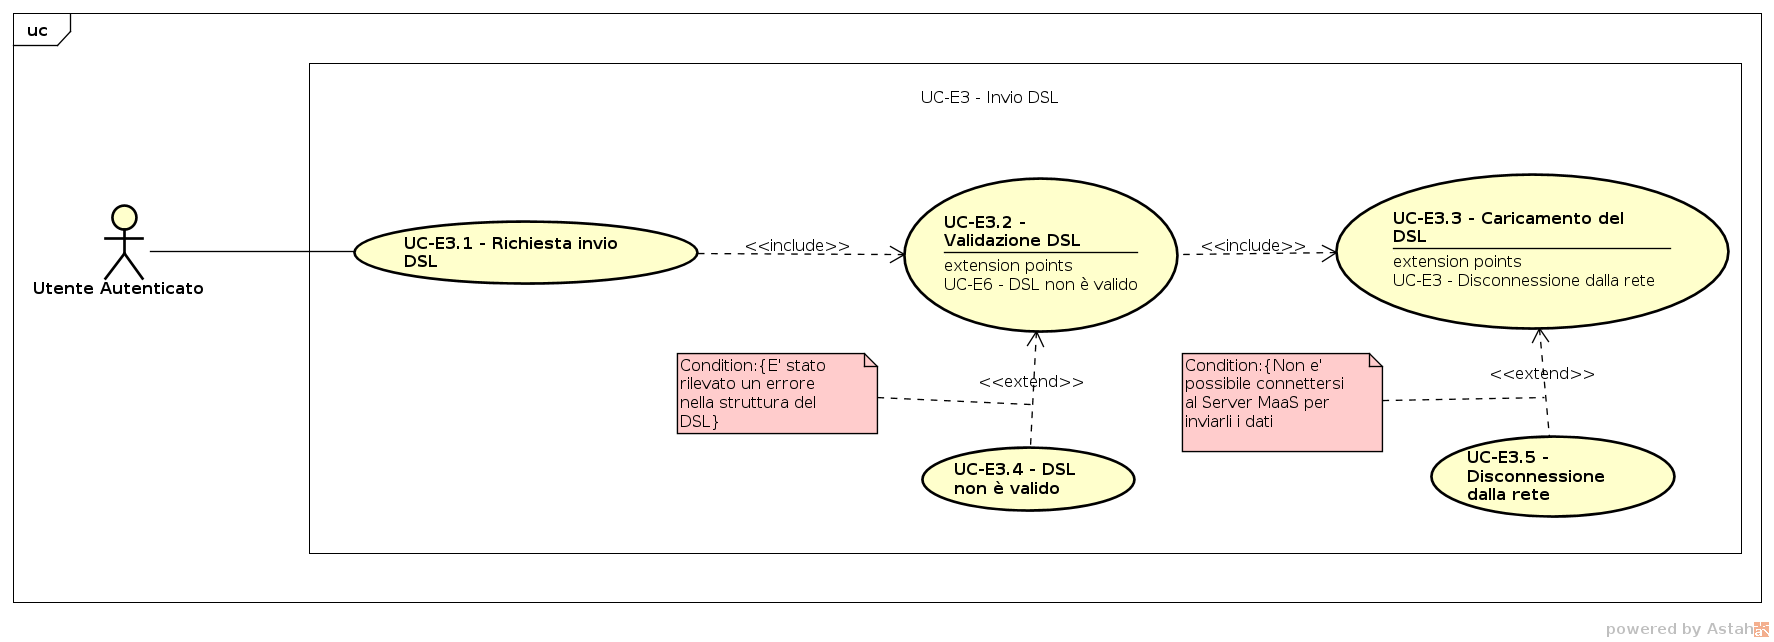
\includegraphics[width=12cm]{res/img/UCEditor/UC-E3}
      \caption{UC-E3 - Salvataggio DSL}
      \end{center} 
    \end{figure}

    %Tabella 
    \begin{center}
      \bgroup
      \def\arraystretch{1.8}     
      \begin{longtable}{  p{3.5cm} | p{8cm} } 
        
        \hline
        \multicolumn{2}{ | c | }{ \cellcolor[gray]{0.9} \textbf{UC-E3 - Salvataggio DSL}} \\ 
        \hline
        
        \textbf{Attori Primari} & Utente Autenticato, Ospite, Membro, Admin, Owner \\ 
        \textbf{Scopo e Descrizione} & Il sistema fornisce una modalit\`a di salvataggio per i DSL definiti da un utente. \\ 
        
        \textbf{Precondizioni}  & L'utente visualizza l'editor e ha creato un DSL valido da salvare. \\ 
        
        \textbf{Postcondizioni} & Il DSL \`e stato memorizzato con successo nel sistema. \\ 
        \textbf{Scenario Principale} & 1. L'utente richiede il salvataggio del DSL. (UC-E3.1) 
      \end{longtable}
      \egroup
    \end{center}
\subsubsection{UC-E3.1}

    %Tabella 
    \begin{center}
      \bgroup
      \def\arraystretch{1.8}     
      \begin{longtable}{  p{3.5cm} | p{8cm} } 
        
        \hline
        \multicolumn{2}{ | c | }{ \cellcolor[gray]{0.9} \textbf{UC-E3.1 - Richiedere il salvataggio del DSL}} \\ 
        \hline
        
        \textbf{Attori Primari} & Utente Autenticato, Ospite, Membro, Admin, Owner \\ 
        \textbf{Scopo e Descrizione} & L'utente chiede all'applicazione di eseguire le operazioni necessarie affinch\`e il DSL venga salvato ed eseguito con successo. \\ 
        
        \textbf{Precondizioni}  & L'utente visualizza l'editor e ha definito un DSL\\ 
        
        \textbf{Postcondizioni} & Il sistema ha preso in carico la richiesta di salvataggio del DSL.
      \end{longtable}
      \egroup
    \end{center}
\subsubsection{UC-E3.2}

    %Tabella 
    \begin{center}
      \bgroup
      \def\arraystretch{1.8}     
      \begin{longtable}{  p{3.5cm} | p{8cm} } 
        
        \hline
        \multicolumn{2}{ | c | }{ \cellcolor[gray]{0.9} \textbf{UC-E3.2 - Validazione del DSL}} \\ 
        \hline
        
        \textbf{Scopo e Descrizione} & Il sistema esegue i controlli di validazione per il DSL creato. \\ 
        
        \textbf{Precondizioni}  & L'utente ha fatto richiesta di salvataggio del DSL \\ 
        
        \textbf{Postcondizioni} & Il DSL \`e stato correttamente validato. \\ 
        \textbf{Estensioni} & 1. Il DSL non \`e valido (UC-E3.4)
      \end{longtable}
      \egroup
    \end{center}
    
    
\subsubsection{UC-E3.3}

    %Tabella 
    \begin{center}
      \bgroup
      \def\arraystretch{1.8}     
      \begin{longtable}{  p{3.5cm} | p{8cm} } 
        
        \hline
        \multicolumn{2}{ | c | }{ \cellcolor[gray]{0.9} \textbf{UC-E3.3 - Memorizzazione del DSL}} \\ 
        \hline
        
         \textbf{Scopo e Descrizione} &  il sistema esegue la procedura di memorizzazione del DSL \\ 
        
        \textbf{Precondizioni}  & Il DSL in input deve essere valido \\ 
        
        \textbf{Postcondizioni} & Il DSL \`e stato correttamente memorizzato al sistema \\ 
      \end{longtable}
      \egroup
    \end{center}
\subsubsection{UC-E3.4}

    %Tabella 
    \begin{center}
      \bgroup
      \def\arraystretch{1.8}     
      \begin{longtable}{  p{3.5cm} | p{8cm} } 
        
        \hline
        \multicolumn{2}{ | c | }{ \cellcolor[gray]{0.9} \textbf{UC-E3.4 - DSL non `e valido}} \\ 
        \hline
        
        \textbf{Scopo e Descrizione} & Il sistema fornisce un messaggio di errore che evidenzia i punti del DSL non validi \\ 
        
        \textbf{Precondizioni}  & Il DSL non \`e corretto \\ 
        
        \textbf{Postcondizioni} & L'utente \`e stato avvisato tramite un messaggio della presenza di errori nel DSL.
      \end{longtable}
      \egroup
    \end{center}
